\documentclass[11pt,a4paper]{article}

\usepackage[utf8]{inputenc}
\usepackage[margin=1in]{geometry}
\usepackage{amsmath,amssymb,amsfonts,bm}
\usepackage{graphicx}
\graphicspath{{../img/}{./}{img/}}
\usepackage{booktabs}
\usepackage{array}
\usepackage{xcolor}
\usepackage{fancyhdr}
\usepackage{tcolorbox}
\usepackage{listings}
\usepackage{microtype}
\usepackage{hyperref}

% Define palette
\definecolor{primaryblue}{RGB}{24, 76, 120}
\definecolor{secondaryblue}{RGB}{41, 128, 185}
\definecolor{darkgray}{RGB}{44, 62, 80}
\definecolor{lightgray}{RGB}{245, 247, 250}
\definecolor{bordergray}{RGB}{200, 205, 210}
\definecolor{codegreen}{RGB}{39, 174, 96}
\definecolor{codecomment}{RGB}{127, 140, 141}
\definecolor{codekeyword}{RGB}{142, 68, 173}

% Hyperref setup
\hypersetup{
    colorlinks=true,
    linkcolor=primaryblue,
    citecolor=primaryblue,
    urlcolor=secondaryblue,
    pdftitle={Lecture 1: AI/ML Foundations and Closed-Loop Control for Particle Accelerators},
    pdfauthor={Chong Shik Park, Ph.D.}
}

% Header and Footer
\pagestyle{fancy}
\fancyhf{}
\fancyhead[L]{\small\color{darkgray}\textbf{AI Applications in Accelerators Tutorial \& Mini-Hackathon}}
\fancyhead[R]{\small\color{darkgray}Lecture Notes}
\fancyfoot[L]{\small\color{darkgray}Lecture 1: AI/ML Foundations \& Closed-Loop Control (Chong Shik Park)}
\fancyfoot[R]{\small\thepage}
\renewcommand{\headrulewidth}{0.6pt}
\renewcommand{\footrulewidth}{0.4pt}

% Affiliation command
\newcommand{\affiliation}[1]{{\normalsize\color{darkgray} #1} \\[0.2em]}

% Code Listing Configuration
\lstdefinestyle{pythonstyle}{
    backgroundcolor=\color{lightgray},
    commentstyle=\color{codecomment}\itshape,
    keywordstyle=\color{codekeyword}\bfseries,
    numberstyle=\tiny\color{codecomment},
    stringstyle=\color{codegreen},
    basicstyle=\ttfamily\footnotesize,
    breakatwhitespace=false,
    breaklines=true,
    captionpos=b,
    keepspaces=true,
    numbers=left,
    numbersep=6pt,
    showspaces=false,
    showstringspaces=false,
    showtabs=false,
    tabsize=4,
    frame=single,
    rulecolor=\color{bordergray}
}
\lstset{style=pythonstyle}

% TColorBox Configuration (Unbreakable boxes kept intact on a single page)
\tcbuselibrary{skins,breakable}
\newtcolorbox{infobox}[1][]{
    enhanced,
    colback=lightgray,
    colframe=primaryblue,
    arc=3mm,
    fonttitle=\bfseries\color{white},
    coltitle=white,
    title=#1,
    left=4mm, right=4mm, top=3mm, bottom=3mm,
    boxrule=0.8pt,
    unbreakable
}

\begin{document}

% Title Banner
\begin{center}
    {\LARGE\bfseries\color{primaryblue} Lecture 1: AI/ML Foundations and Closed-Loop Control for Particle Accelerators} \\[0.8em]
    {\large\color{darkgray} Physics Foundations, Neural Surrogates, Reinforcement Learning, and Bayesian Optimization} \\[0.5em]
    \rule{\textwidth}{1.2pt} \\[0.5em]
    \textbf{Chong Shik Park, Ph.D.} \\[0.3em]
    \affiliation{Department of Accelerator Science, Korea University, Sejong 30019, Republic of Korea}
    \affiliation{Center for Accelerator Research, Korea University, Sejong 30019, Republic of Korea}
    \vspace{0.2em}
    {\small\color{darkgray} November 19, 2026}
\end{center}

\vspace{0.5em}

\begin{abstract}
Modern particle accelerator facilities operate with thousands of tightly coupled magnet actuators and diagnostics under sub-micron beam stability tolerances. Classical linear feedback systems face fundamental bottlenecks in non-linear regimes where magnetic core saturation and power supply limits degrade control fidelity. This lecture provides the theoretical and computational foundation bridging transverse beam dynamics, Hill's equation, and the Orbit Response Matrix (ORM) with cutting-edge supervised machine learning and reinforcement learning. We explore the design and training of neural surrogate digital twins to model cubic saturation, compare classical singular value decomposition (SVD) with model-based bounded optimization (\texttt{L-BFGS-B}), and investigate physics-informed closed-loop policy agents with adaptive damping for the afternoon Beam Orbit Alignment Mini-Hackathon.
\end{abstract}

\clearpage

\tableofcontents

\clearpage

\section{Introduction: AI Applications in Modern Particle Accelerators}

Over the past decade, Artificial Intelligence (AI) and Machine Learning (ML) have evolved from experimental proofs-of-concept into mission-critical operational tools across modern particle accelerator facilities, including synchrotron light sources, free-electron lasers (XFELs), spallation neutron sources, high-intensity hadron linacs, and energy-frontier colliders~\cite{edelen2020opportunities}. Modern accelerators operate with thousands of distributed, non-linearly coupled magnet actuators, radiofrequency (RF) accelerating stations, and high-rate diagnostic monitors under stringent beam quality and stability demands.

The landscape of AI applications in particle accelerators is broadly categorized into five foundational pillars:
\begin{enumerate}
    \item \textbf{Surrogate Modeling \& Fast Digital Twins~\cite{edelen2020opportunities, edelen2018neural}:}
    High-fidelity numerical particle tracking codes (such as \texttt{ELEGANT}, \texttt{MAD-X}, and \texttt{OPAL}) simulate complex beam dynamics, space-charge forces, and collective effects, but require minutes to hours per run. Deep neural networks (Multi-Layer Perceptrons, Convolutional Networks, and Physics-Informed Neural Networks) learn fast surrogate representations capable of evaluating beamline outcomes in sub-millisecond execution times. These ultra-fast surrogates serve as digital twins for real-time model-predictive control, online trajectory correction, and rapid parametric sensitivity analysis.

    \item \textbf{Multi-Objective Autonomous Optimization \& Tuning~\cite{roussel2023turnkey, edelen2020machine}:}
    Commissioning and daily operations involve optimizing conflicting performance objectives---such as maximizing beam transmission and photon brightness while minimizing transverse emittance and beam halo. Bayesian Optimization (BO) with Gaussian Processes, combined with active learning and exploration-exploitation acquisition functions, enables sample-efficient multi-objective optimization directly on physical machines, converging in dozens of shots compared to thousands of iterations required by brute-force parameter scans.

    \item \textbf{Virtual Diagnostics \& Non-Destructive Phase Space Reconstruction~\cite{emma2021virtual}:}
    Critical beam properties---such as 6D phase space, bunch slice emittance, and femtosecond current profiles---often require interceptive diagnostics (e.g., transverse deflection cavities, wire scanners, or screens) that disrupt or destroy the beam. Virtual diagnostics leverage supervised machine learning to accurately reconstruct unmeasured or destructive bunch characteristics shot-by-shot from non-invasive upstream RF probes, magnet currents, and Beam Position Monitor (BPM) signals.

    \item \textbf{Anomaly Detection, Fault Prediction \& Machine Protection~\cite{tennant2020supervised}:}
    Unscheduled beam downtime in multi-megawatt hadron linacs and synchrotron facilities incurs heavy scientific and operational costs. Unsupervised machine learning (autoencoders, isolation forests) continuously monitors archival and real-time telemetry to detect subtle precursor drift patterns, while deep sequence models predict high-voltage RF breakdowns, ion source dropouts, and superconducting cavity quenches milliseconds before catastrophic failure, triggering proactive mitigation and machine protection interlocks.

    \item \textbf{Agentic AI \& Autonomous Operation Workflows~\cite{hellert2024autonomous}:}
    Moving beyond single-purpose neural networks, modern research explores autonomous agent architectures (such as \textit{Osprey} and LLM-driven scientific agents). These systems integrate large language models with standardized Python control APIs, simulation engines, and diagnostic databases, enabling high-level natural language operational commands (e.g., ``align the transport line orbit and optimize injection efficiency'') to be autonomously planned, validated, and executed under strict domain guardrails.
\end{enumerate}

---

\section{Motivation \& Accelerator Physics Foundations}

\subsection{The Operational Stability Challenge}
In synchrotron light sources, free-electron lasers (XFELs), and medical linacs, particle beam stability must be sustained at sub-micron levels to maintain photon brightness and collision luminosity. 

Transverse orbit stability is equally vital in \textbf{hadron linacs} (high-intensity proton and heavy-ion linear accelerators). In modern high-power hadron facilities, uncorrected beam trajectory offsets through accelerating RF cavities and focusing quadrupoles induce strong non-linear space-charge forces, emittance growth, and halo formation. Because high-intensity hadron beams carry enormous beam power, even minute fractional beam losses (exceeding $1\text{ W/m}$ or $10^{-5}$ of total current) induce severe structural radioactivation, prohibiting hands-on maintenance and risking superconducting cavity quenches or vacuum chamber damage.

Orbit distortions arise from multiple sources:
\begin{itemize}
    \item \textbf{Slow Drifts:} Thermal expansion of girders, diurnal ambient temperature shifts, and ground motion.
    \item \textbf{Dynamic Jitter:} Mechanical vibration from cooling water pumps, cryocoolers, and power supply ripple.
    \item \textbf{High Actuator Coupling:} Deflecting a single dipole corrector causes betatron wave propagation across the entire transport line.
\end{itemize}

\subsection{Transverse Beam Dynamics \& Hill's Equation}
In an uncoupled linear transport channel, the transverse displacement $x(s)$ as a function of path length $s$ is governed by \textbf{Hill's Equation}~\cite{wiedemann2015particle}:
\begin{equation}
    \frac{d^2 x(s)}{ds^2} + K(s) x(s) = 0
\end{equation}
where $K(s) = \frac{e}{p} \frac{\partial B_y(s)}{\partial x}$ represents the alternating quadrupole focusing strength ($K > 0$ for horizontal focusing `QF', $K < 0$ for defocusing `QD').

The closed-form betatron solution is given by:
\begin{equation}
    x(s) = \sqrt{\epsilon \beta(s)} \cos\left( \psi(s) + \phi_0 \right)
\end{equation}
where $\beta(s)$ is the Courant-Snyder beta function, $\psi(s) = \int_0^s \frac{d\bar{s}}{\beta(\bar{s})}$ is the betatron phase advance, and $\nu = \frac{1}{2\pi} \oint \frac{ds}{\beta(s)}$ is the betatron tune.

\subsection{Derivation of the Orbit Response Matrix (ORM)}
When an angular kick $\theta_j = \Delta x'_j = \frac{e B L}{p}$ is applied by a dipole corrector at longitudinal position $s_j$, the transverse displacement registered at a downstream Beam Position Monitor (BPM) at position $s_i$ is linearly proportional to the kick angle:
\begin{equation}
    R_{ij} = \frac{\Delta x(s_i)}{\theta_j} = \frac{\sqrt{\beta(s_i)\beta(s_j)}}{2 \sin(\pi \nu)} \cos\left( |\psi(s_i) - \psi(s_j)| - \pi \nu \right)
\end{equation}
For $M$ BPMs and $N$ dipole steerers, the linear response is encapsulated by the matrix $\mathbf{R} \in \mathbb{R}^{N \times M}$~\cite{minty2003measurement}:
\begin{equation}
    \mathbf{Y}_{\text{linear}} = \mathbf{I} \cdot \mathbf{R}
\end{equation}
where $\mathbf{I} = [I_1, I_2, \dots, I_N]$ represents the corrector current vector.

\begin{figure}[t!]
\centering
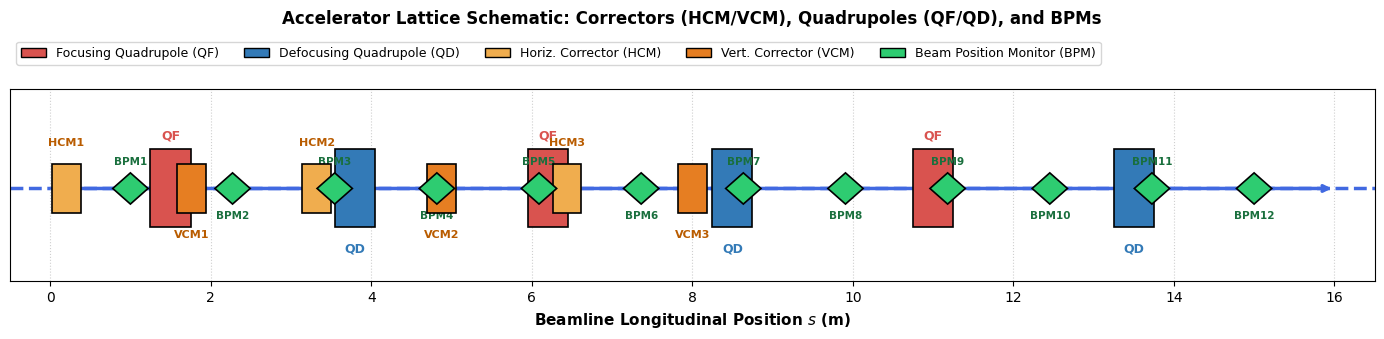
\includegraphics[width=0.95\textwidth]{beamline.png}
\caption{Schematic diagram of the 15-meter accelerator transport section showing alternating focusing (QF, red) and defocusing (QD, blue) quadrupoles, 6 dipole steerers (HCM/VCM), and 12 Beam Position Monitors.}
\label{fig:beamline}
\end{figure}

\subsection{Mini-Hackathon Lattice Geometry \& Realistic Non-Linearities}
The mini-hackathon benchmark lattice (Figure~\ref{fig:beamline}) models a 15-meter transport line:
\begin{itemize}
    \item \textbf{Actuators:} 6 dipole steerers (3 Horizontal `HCM1--3', 3 Vertical `VCM1--3') bounded in $[-5.0\text{ A}, +5.0\text{ A}]$, with single-step adjustments clipped to $[-0.8\text{ A}, +0.8\text{ A}]$.
    \item \textbf{Diagnostics:} 12 Beam Position Monitors ($s = 1.0\text{ m}$ to $15.0\text{ m}$) reading beam displacement in millimeters.
    \item \textbf{Magnetic Core Saturation:} Ferromagnetic saturation at higher excitation currents induces non-linear cubic rolloff:
    \begin{equation}
        \mathbf{Y}_{\text{sat}} = - 0.015 \cdot (\mathbf{I}^3 \cdot \mathbf{R})
    \end{equation}
    \item \textbf{Initial Misalignment Distortion ($\mathbf{Y}_0$):} Quadrupole displacement errors drawn per episode:
    \begin{equation}
        Y_{0, k} = A_1 \sin\left(\frac{2\pi s_k}{\lambda_1} + \phi_1\right) + A_2 \cos\left(\frac{2\pi s_k}{\lambda_2} + \phi_2\right)
    \end{equation}
    producing initial orbit errors between $0.4\text{ mm}$ and $1.1\text{ mm}$ RMS.
    \item \textbf{Gaussian Measurement Noise:} Sensor electronics introduce random noise $\boldsymbol{\epsilon} \sim \mathcal{N}(0, \sigma^2)$, with $\sigma = 0.010\text{ mm}$ ($10\ \mu\text{m}$).
\end{itemize}

The complete physical forward response equation is:
\begin{equation}
    \mathbf{Y} = \mathbf{I} \cdot \mathbf{R} - 0.015 \cdot (\mathbf{I}^3 \cdot \mathbf{R}) + \mathbf{Y}_0 + \boldsymbol{\epsilon}
\end{equation}

---

\section{Machine Learning Fundamentals \& Neural Surrogate Modeling}

\subsection{Machine Learning Taxonomy in Accelerators}
Machine Learning (ML) algorithms automatically extract functional mappings from numerical tracking simulations or machine archives without requiring explicit analytical re-derivation. In accelerator operations, ML encompasses three main paradigms:
\begin{itemize}
    \item \textbf{Supervised Learning:} Learning a continuous regression mapping $\mathbf{Y} = f(\mathbf{X})$ from actuator magnet currents $\mathbf{X}$ to beam diagnostic offsets $\mathbf{Y}$. This forms the foundation of \textbf{Surrogate Modeling / Digital Twins}.
    \item \textbf{Unsupervised Learning:} Uncovering latent structures in unlabelled data (e.g., PCA for betatron mode decomposition, autoencoders for anomaly detection).
    \item \textbf{Reinforcement Learning (RL):} Training an agent policy $\pi(a|s)$ through environmental interaction to maximize cumulative reward for \textbf{Autonomous Closed-Loop Control}.
\end{itemize}

\subsection{Foundational ML Paradigms: Forward Supervised Learning vs. Reinforcement Learning}
In developing autonomous beam alignment algorithms, accelerator engineers rely primarily on two complementary paradigms: \textbf{Forward Supervised Learning} (training a digital twin surrogate of the accelerator to be inverted) and \textbf{Reinforcement Learning} (training a closed-loop policy agent that directly interacts with the machine). Figure~\ref{fig:sl_vs_rl} illustrates their distinct architectural workflows.

\begin{figure}[t!]
\centering
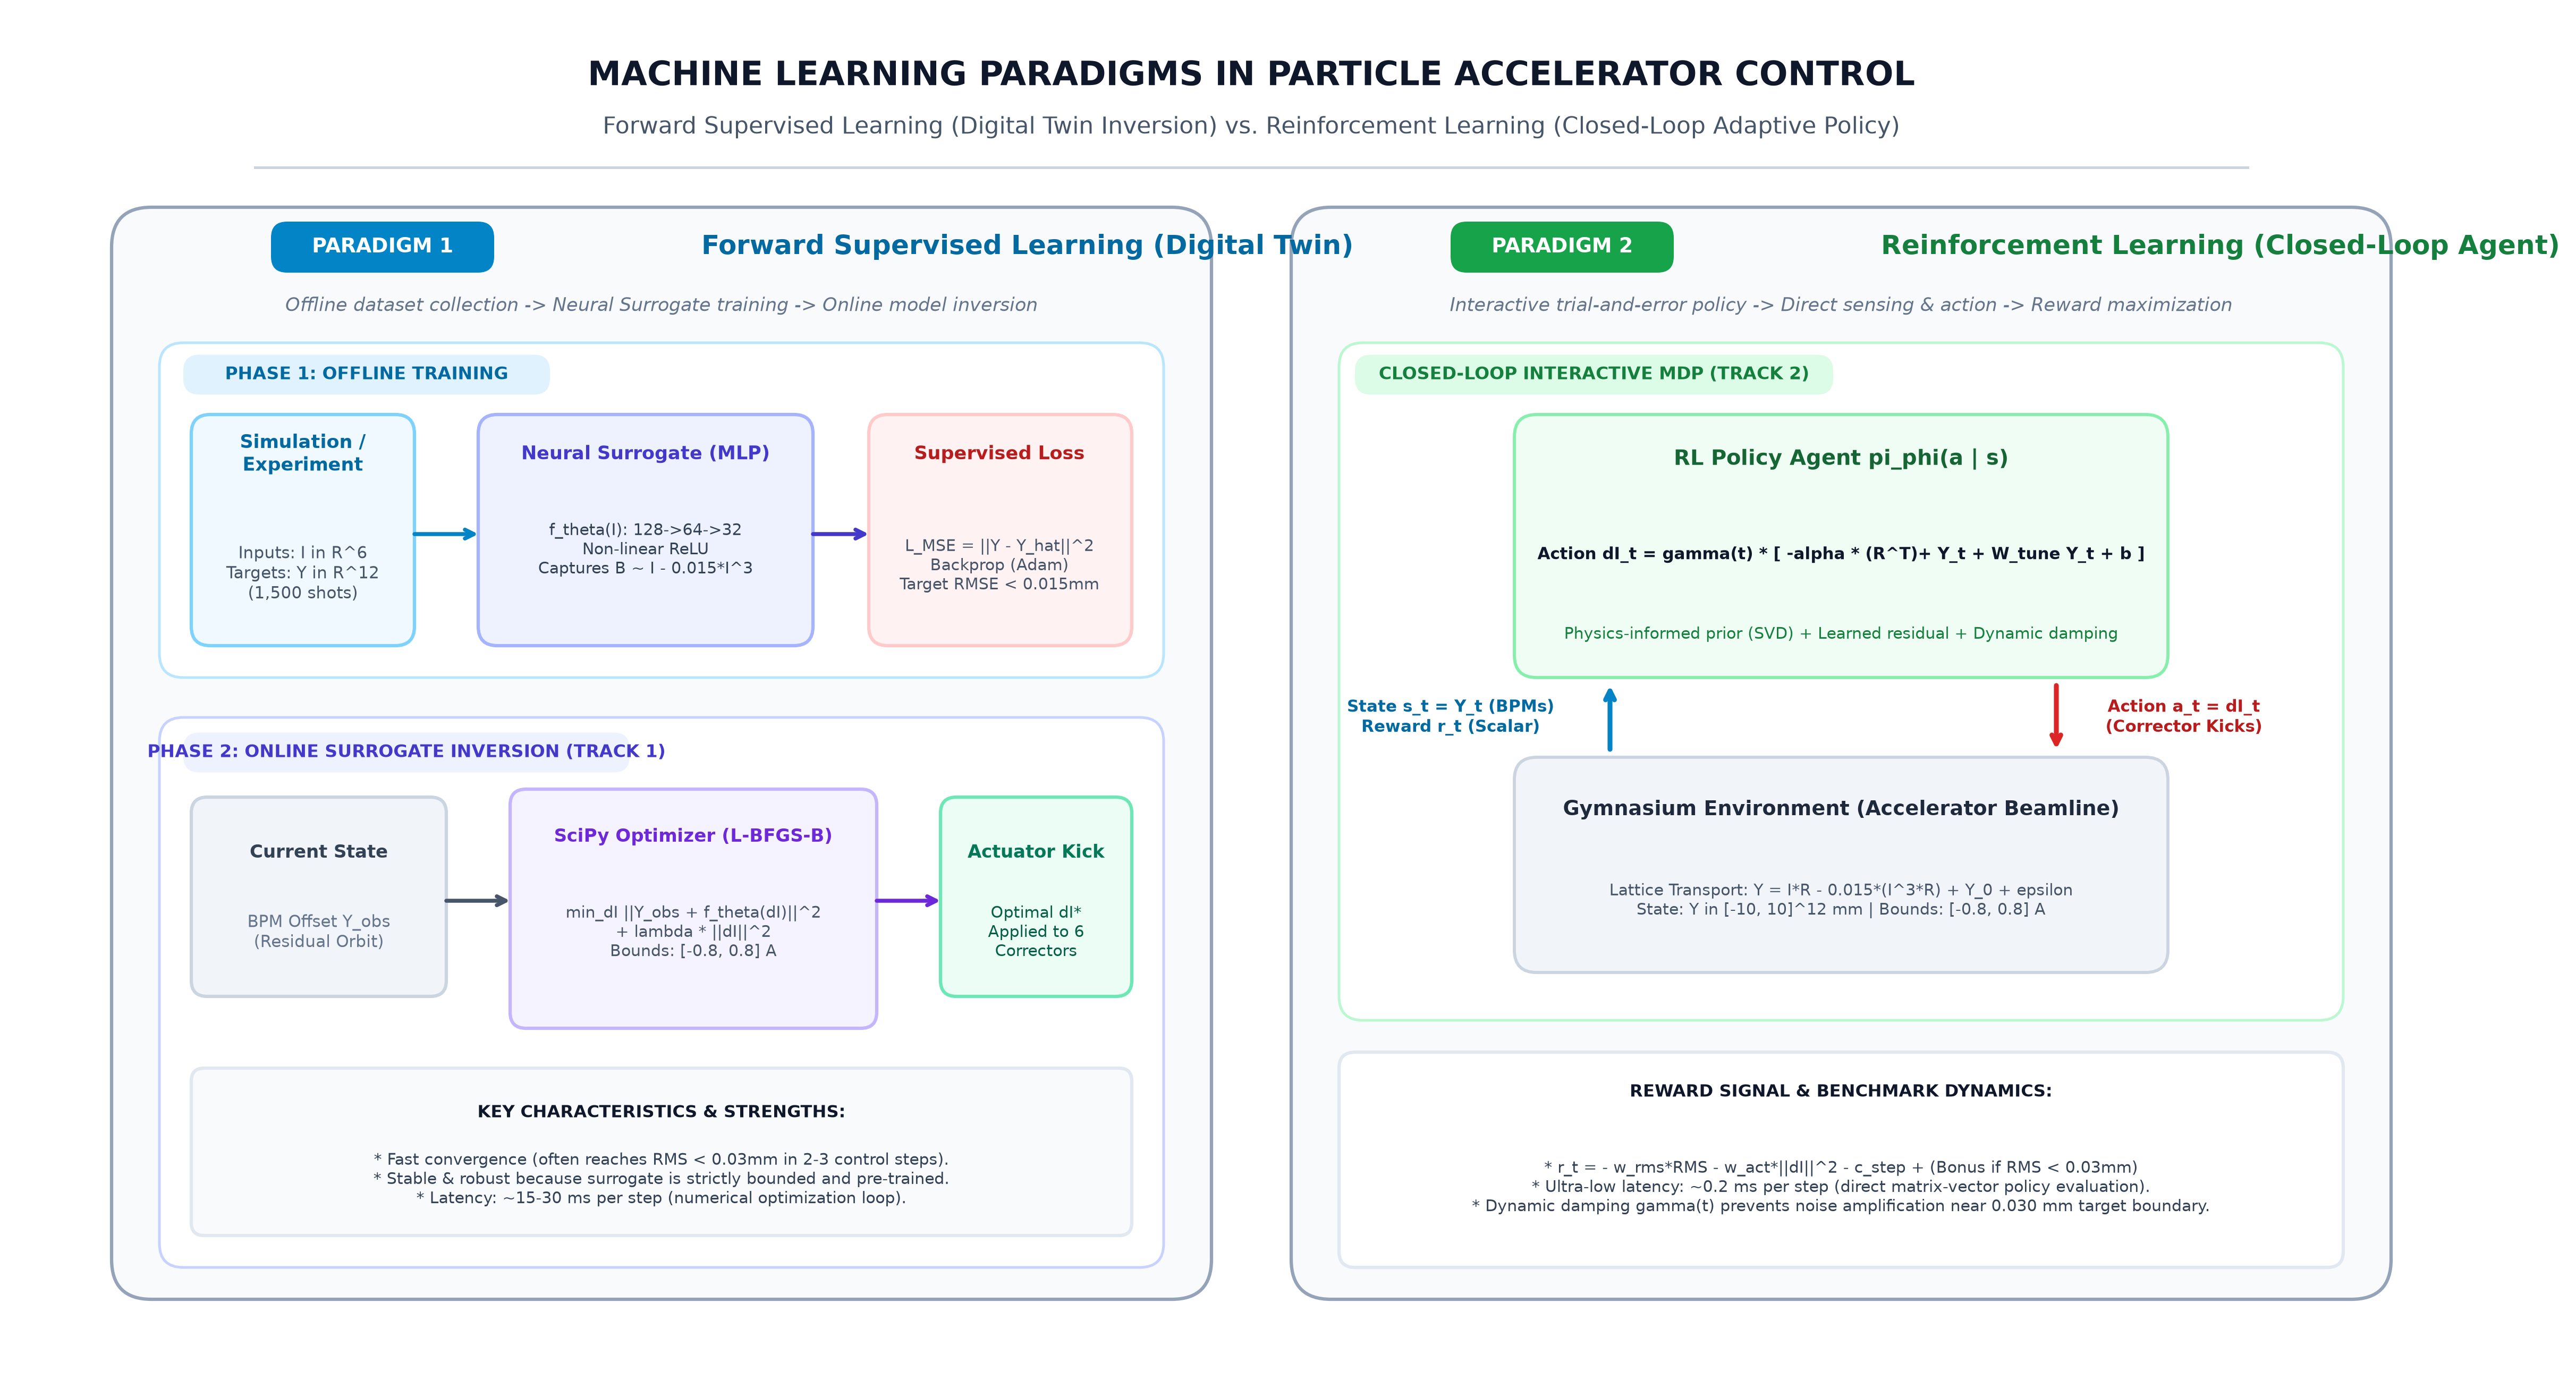
\includegraphics[width=0.98\textwidth]{forward_sl_and_rl_schematic.png}
\caption{Architectural comparison between Forward Supervised Learning (Surrogate Digital Twin \& Inversion, Track 1) and Reinforcement Learning (Closed-Loop Policy Interaction, Track 2) for particle accelerator orbit control.}
\label{fig:sl_vs_rl}
\end{figure}

\subsubsection{Forward Supervised Learning: Digital Twin Surrogate \& Inversion (Track 1)}
In Forward Supervised Learning, the model learns the predictive forward response mapping $\mathbf{I} \mapsto \mathbf{Y}$ from passive, pre-recorded tracking simulation datasets:
\begin{enumerate}
    \item \textbf{Offline Dataset Generation:} We sample $N$ random corrector current vectors $\mathbf{I} \in \mathbb{R}^6$ across operating ranges (e.g., $[-3.0\text{ A}, +3.0\text{ A}]$) and evaluate their transverse displacements $\mathbf{Y} \in \mathbb{R}^{12}$ across all 12 BPMs, yielding dataset $\mathcal{D} = \{(\mathbf{I}^{(i)}, \mathbf{Y}^{(i)})\}_{i=1}^N$.
    \item \textbf{Surrogate Model Training:} A deep neural network (e.g. Multi-Layer Perceptron $f_{\boldsymbol{\theta}}$ with layers $128 \rightarrow 64 \rightarrow 32$) is trained to minimize the Mean Squared Error (MSE) loss:
    \begin{equation}
        \mathcal{L}_{\text{MSE}}(\boldsymbol{\theta}) = \frac{1}{N} \sum_{i=1}^N \left\| \mathbf{Y}^{(i)} - f_{\boldsymbol{\theta}}(\mathbf{I}^{(i)}) \right\|_2^2
    \end{equation}
    Through Adam backpropagation, the neural surrogate captures non-linear magnetic core saturation $B(I) \approx I - 0.015 \cdot I^3$ down to the $0.010\text{ mm}$ diagnostic noise floor.
    \item \textbf{Online Inversion for Beam Alignment:} During beam operations, observed orbit distortions $\mathbf{Y}_{\text{obs}}$ are corrected by solving an online bounded minimization problem:
    \begin{equation}
        \Delta \mathbf{I}^* = \arg\min_{\Delta \mathbf{I}} \left\| \mathbf{Y}_{\text{obs}} + f_{\boldsymbol{\theta}}(\Delta \mathbf{I}) \right\|_2^2 + \lambda \|\Delta \mathbf{I}\|_2^2 \quad \text{subject to } \Delta \mathbf{I} \in [-0.8\text{ A}, +0.8\text{ A}]^6
    \end{equation}
    Because the surrogate captures soft saturation, this approach converges in as few as 2 to 3 iterations.
\end{enumerate}

\subsubsection{Reinforcement Learning: Closed-Loop Policy Control (Track 2)}
In Reinforcement Learning (RL), orbit steering is formulated as a Markov Decision Process (MDP) $(\mathcal{S}, \mathcal{A}, \mathcal{P}, \mathcal{R}, \gamma)$:
\begin{enumerate}
    \item \textbf{State Space ($\mathcal{S}$):} Transverse beam offsets measured at 12 BPM stations: $\mathbf{s}_t = \mathbf{Y}_t \in [-10.0\text{ mm}, +10.0\text{ mm}]^{12}$.
    \item \textbf{Action Space ($\mathcal{A}$):} Corrector kick delta currents: $\mathbf{a}_t = \Delta \mathbf{I}_t \in [-0.8\text{ A}, +0.8\text{ A}]^6$.
    \item \textbf{Environment Dynamics ($\mathcal{P}$):} Physical transport law including betatron optics, core saturation, misalignment drift $\mathbf{Y}_0$, and sensor noise $\boldsymbol{\epsilon}$:
    \begin{equation}
        \mathbf{I}_{t+1} = \text{clip}(\mathbf{I}_t + \mathbf{a}_t, -5.0, +5.0)\text{ A}, \quad \mathbf{s}_{t+1} = \mathbf{I}_{t+1} \cdot \mathbf{R} - 0.015 \cdot (\mathbf{I}_{t+1}^3 \cdot \mathbf{R}) + \mathbf{Y}_0 + \boldsymbol{\epsilon}
    \end{equation}
    \item \textbf{Reward Signal ($\mathcal{R}$):} Scalar feedback rewarding alignment precision and penalizing actuator effort and steps:
    \begin{equation}
        r_t = - w_{\text{rms}} \cdot \text{RMS}_{t+1} - w_{\text{act}} \cdot \|\mathbf{a}_t\|_2^2 - c_{\text{step}} + (B_{\text{success}} \text{ if terminated else } 0.0)
    \end{equation}
    \item \textbf{Physics-Informed Prior \& Adaptive Damping:} High-performance policies synthesize an analytical pseudo-inverse prior with learned non-linear residual compensation and dynamic step cooling:
    \begin{equation}
        \Delta \mathbf{I}_t = \gamma(t) \cdot \left[ - \alpha (\mathbf{R}^T)^\dagger \mathbf{Y}_t + \mathbf{W}_{\text{tune}} \mathbf{Y}_t + \mathbf{b} \right], \quad \gamma(t) = \frac{1.0}{1.0 + 0.03 \cdot t}
    \end{equation}
    This enables direct policy execution in single forward passes ($\approx 0.2\text{ ms}$ latency).
\end{enumerate}

\subsubsection{Comparative Architectural Analysis}
Table~\ref{tab:sl_vs_rl} summarizes the fundamental operational differences between the two paradigms.

\begin{table}[h!]
\centering
\small
\begin{tabular}{p{3.5cm} p{5.5cm} p{5.5cm}}
\toprule
\textbf{Dimension} & \textbf{Forward Supervised Learning (Track 1)} & \textbf{Reinforcement Learning (Track 2)} \\
\midrule
\textbf{Primary Goal} & Accurate physical predictive twin ($\hat{\mathbf{Y}} = f_{\boldsymbol{\theta}}(\mathbf{I})$) & Optimal closed-loop action policy ($\mathbf{a}_t = \pi_{\boldsymbol{\phi}}(\mathbf{s}_t)$) \\
\textbf{Data Source} & Offline passive sampling across grid & Online interactive rollouts in environment \\
\textbf{Training Signal} & Ground-truth diagnostic vectors $\mathbf{Y}$ & Scalar reward feedback $r_t$ \\
\textbf{Objective} & Minimize MSE / RMSE error & Maximize cumulative return $\mathbb{E}[\sum \gamma^t r_t]$ \\
\textbf{Control Mechanism} & Forward twin + SciPy \texttt{L-BFGS-B} solver & Direct feedback policy evaluation \\
\textbf{Execution Latency} & $\approx 15 - 30\text{ ms}$ per step & $\approx 0.2\text{ ms}$ per step \\
\textbf{Sample Efficiency} & High ($1,500$ shots trains full model) & Moderate to high (with physics priors) \\
\textbf{Safety Handling} & Explicit box constraints in optimizer & Hardware action clipping \& damping \\
\bottomrule
\end{tabular}
\caption{Comparison of Forward Supervised Learning vs.\ Closed-Loop Reinforcement Learning for accelerator control.}
\label{tab:sl_vs_rl}
\end{table}

\subsection{The Artificial Neuron: Mathematical Formulation}
The fundamental atom of a neural network is the \textbf{artificial neuron} (perceptron):
\begin{enumerate}
    \item \textbf{Linear Combination (Pre-Activation):}
    \begin{equation}
        z = \sum_{i=1}^n w_i x_i + b = \mathbf{w}^T \mathbf{x} + b
    \end{equation}
    where $\mathbf{w} \in \mathbb{R}^n$ denotes the trainable synaptic weights, $\mathbf{x} \in \mathbb{R}^n$ is the input feature vector, and $b \in \mathbb{R}$ is the scalar bias shifting the firing threshold.
    
    \item \textbf{Non-Linear Mapping (Post-Activation):}
    \begin{equation}
        a = \sigma(z) = \sigma(\mathbf{w}^T \mathbf{x} + b)
    \end{equation}
    where $\sigma(\cdot)$ is the activation function.
\end{enumerate}

\subsection{Why Non-Linear Activation Functions are Essential}
\begin{infobox}[The Collapse of Deep Linear Networks]
If all activation functions were linear identities ($\sigma(z) = z$), stacking $L$ sequential layers would yield:
\begin{equation}
    \hat{\mathbf{Y}} = \mathbf{W}_3 (\mathbf{W}_2 (\mathbf{W}_1 \mathbf{x} + \mathbf{b}_1) + \mathbf{b}_2) + \mathbf{b}_3 = (\mathbf{W}_3 \mathbf{W}_2 \mathbf{W}_1) \mathbf{x} + \mathbf{b}_{\text{net}} = \mathbf{W}_{\text{eff}} \mathbf{x} + \mathbf{b}_{\text{net}}
\end{equation}
A multi-layer linear network collapses mathematically into a \textbf{single linear matrix} $\mathbf{W}_{\text{eff}}$, offering no more expressive capacity than the classical linear Orbit Response Matrix $\mathbf{R}$.
\end{infobox}

Non-linear activation functions enable neural networks to act as Universal Function Approximators:
\begin{itemize}
    \item \textbf{Sigmoid:} $\sigma(z) = \frac{1}{1 + e^{-z}} \in (0, 1)$. Suffers from vanishing gradients when $|z| \gg 0$, halting weight updates during backpropagation.
    \item \textbf{Hyperbolic Tangent ($\tanh$):} $\tanh(z) = \frac{e^z - e^{-z}}{e^z + e^{-z}} \in (-1, 1)$. Zero-centered, but still prone to gradient saturation.
    \item \textbf{Rectified Linear Unit (ReLU):}
    \begin{equation}
        \text{ReLU}(z) = \max(0, z) = \begin{cases} z & \text{if } z > 0 \\ 0 & \text{if } z \le 0 \end{cases}
    \end{equation}
    \textbf{Why ReLU is standard in accelerator surrogates:}
    \begin{itemize}
        \item Constant unit derivative $\frac{d}{dz}\text{ReLU}(z) = 1.0$ for $z > 0$, completely preventing gradient vanishing.
        \item Extremely fast forward and backward passes without exponential function evaluation.
        \item Induces sparse representations by zeroing negative activations.
    \end{itemize}
\end{itemize}

\subsection{Multi-Layer Perceptron (MLP) Topology: Layers \& Information Flow}
A Multi-Layer Perceptron (MLP) organizes interconnected neurons into sequential layers (Figure~\ref{fig:mlp_schematic}):

\begin{figure}[h!]
\centering
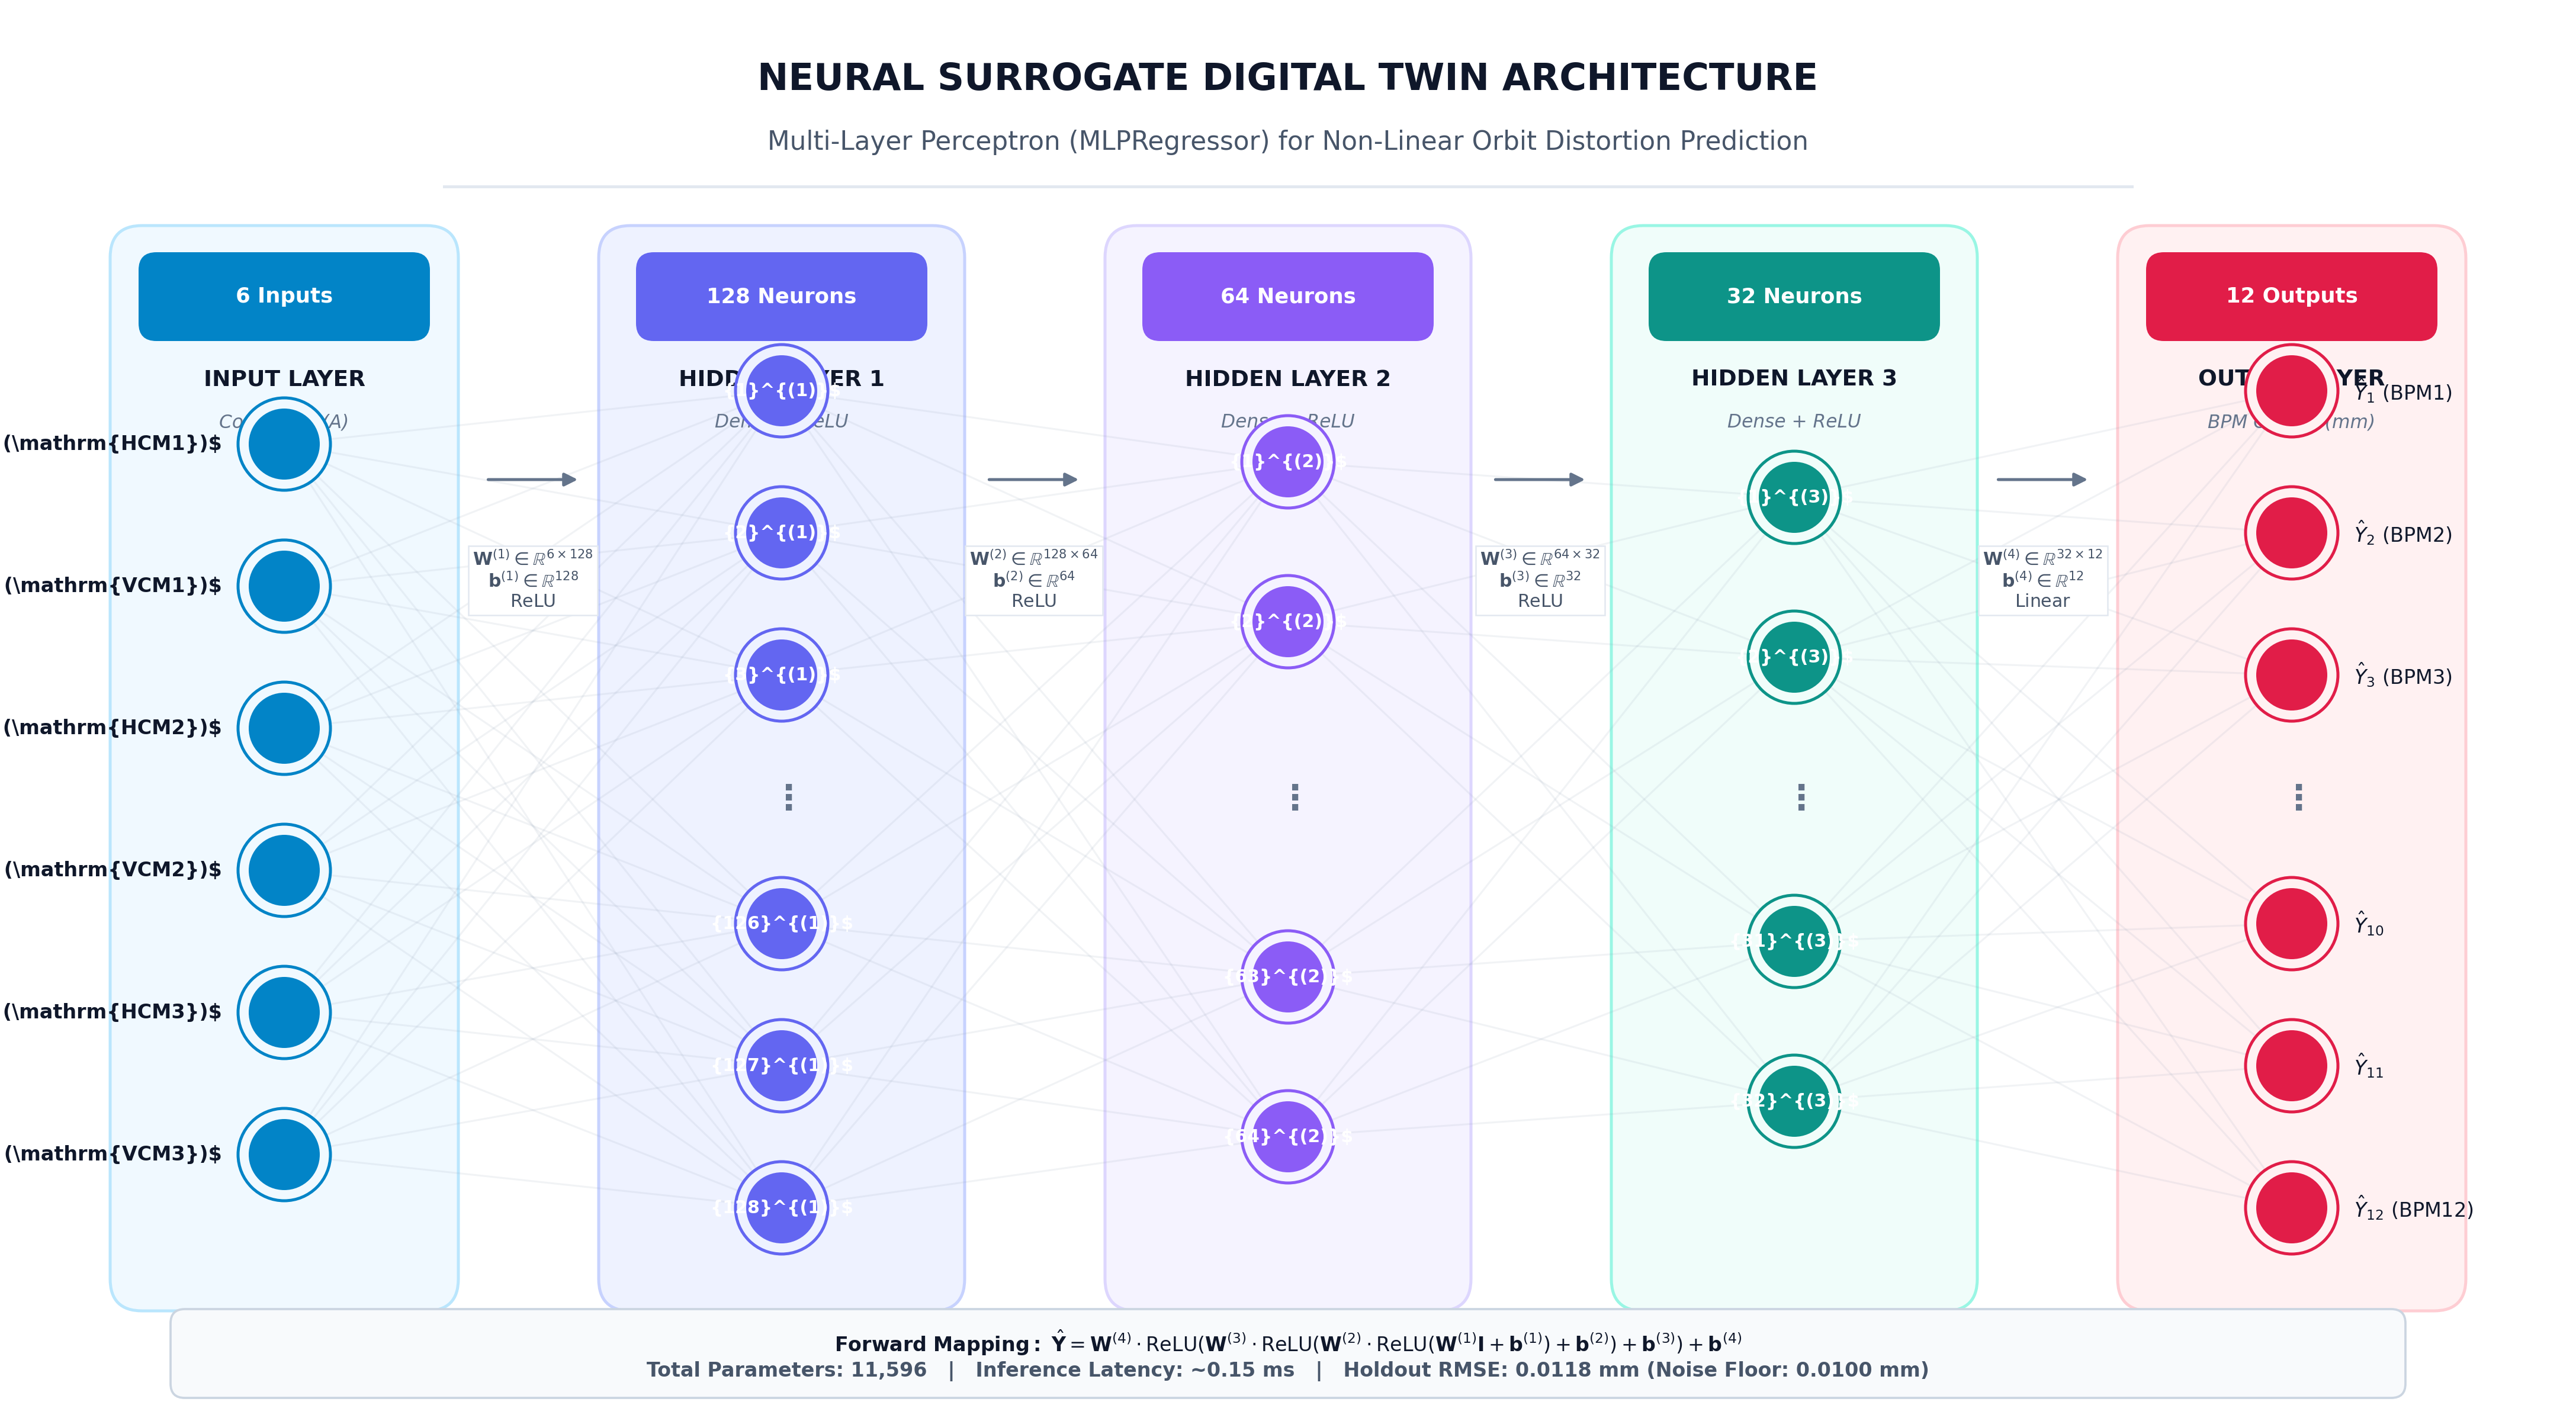
\includegraphics[width=0.90\textwidth]{mlp_schematic.png}
\caption{Architecture of the Multi-Layer Perceptron (MLP) neural surrogate digital twin, mapping 6 dipole corrector currents to 12 BPM transverse orbit offsets through three hidden layers (128, 64, 32 units) with ReLU activations.}
\label{fig:mlp_schematic}
\end{figure}

\begin{itemize}
    \item \textbf{Input Layer ($\mathbb{R}^6$):} Ingests physical magnet actuator setpoints (the 6 corrector currents $I_1, \dots, I_6$).
    \item \textbf{Hidden Layers ($\mathbb{R}^{128} \rightarrow \mathbb{R}^{64} \rightarrow \mathbb{R}^{32}$):} Progressive hierarchical feature representations. Each layer computes:
    \begin{equation}
        \mathbf{h}^{(l)} = \text{ReLU}\left( \mathbf{W}^{(l)} \mathbf{h}^{(l-1)} + \mathbf{b}^{(l)} \right)
    \end{equation}
    \item \textbf{Output Layer ($\mathbb{R}^{12}$):} Linear projection predicting the 12 Beam Position Monitor readings ($\hat{Y}_1, \dots, \hat{Y}_{12}$).
\end{itemize}

\subsection{Loss Functions, Loss Rates \& Metrics: MSE vs.\ RMSE}
Network parameters are trained by minimizing an objective loss function:
\begin{enumerate}
    \item \textbf{Mean Squared Error (MSE) Loss:}
    \begin{equation}
        \mathcal{L}_{\text{MSE}}(\boldsymbol{\theta}) = \frac{1}{N \cdot M} \sum_{i=1}^N \sum_{j=1}^M \left( Y_{i,j} - \hat{Y}_{i,j}(\boldsymbol{\theta}) \right)^2
    \end{equation}
    Smoothly differentiable, penalizing large orbit outliers quadratically.
    
    \item \textbf{Root Mean Squared Error (RMSE) Evaluation Metric:}
    \begin{equation}
        \text{RMSE} = \sqrt{\mathcal{L}_{\text{MSE}}} = \sqrt{\frac{1}{N \cdot M} \sum_{i=1}^N \sum_{j=1}^M \left( Y_{i,j} - \hat{Y}_{i,j} \right)^2}
    \end{equation}
    \textbf{Why RMSE is the preferred metric in beam physics:} It preserves the original physical measurement units (\textbf{millimeters}) and directly reflects accelerator beam orbit distortion standards.
\end{enumerate}

\subsection{Optimization Algorithms: Gradient Descent \& The Adam Optimizer}
During backpropagation, loss gradients $\nabla_{\boldsymbol{\theta}} \mathcal{L}$ are propagated backward to update weights:
\begin{enumerate}
    \item \textbf{Stochastic Gradient Descent (SGD):} $\boldsymbol{\theta}_{t+1} = \boldsymbol{\theta}_t - \eta \nabla_{\boldsymbol{\theta}} \mathcal{L}$, where $\eta$ is the \textbf{learning rate}. High learning rates risk divergence; low learning rates cause stagnation.
    \item \textbf{The Adam Optimizer (Adaptive Moment Estimation):} Combines Momentum (first moment $\mathbf{m}_t$) and RMSprop (second moment $\mathbf{v}_t$):
    \begin{equation}
        \mathbf{m}_t = \beta_1 \mathbf{m}_{t-1} + (1-\beta_1) \mathbf{g}_t, \quad \mathbf{v}_t = \beta_2 \mathbf{v}_{t-1} + (1-\beta_2) \mathbf{g}_t^2
    \end{equation}
    \begin{equation}
        \hat{\mathbf{m}}_t = \frac{\mathbf{m}_t}{1-\beta_1^t}, \quad \hat{\mathbf{v}}_t = \frac{\mathbf{v}_t}{1-\beta_2^t} \implies \boldsymbol{\theta}_{t+1} = \boldsymbol{\theta}_t - \frac{\eta}{\sqrt{\hat{\mathbf{v}}_t} + \epsilon} \hat{\mathbf{m}}_t
    \end{equation}
    Adam automatically scales individual parameter updates, ensuring stable convergence across coupled magnet channels.
\end{enumerate}

\subsection{Dataset Partitioning \& The Bias-Variance Tradeoff}
To prevent memorization of diagnostic noise, data is partitioned into:
\begin{itemize}
    \item \textbf{Training Set (80\%, 1,200 shots):} Used directly for loss gradient computation and parameter updates.
    \item \textbf{Validation Set (Optional):} Monitored across epochs for early stopping before overfitting occurs.
    \item \textbf{Test / Holdout Set (20\%, 300 shots):} Strictly isolated during training to provide an unbiased benchmark on unseen accelerator states.
\end{itemize}
\begin{itemize}
    \item \textbf{Underfitting (High Bias):} Linear models cannot capture the cubic magnetic core saturation.
    \item \textbf{Overfitting (High Variance):} Over-parameterized models memorizing Gaussian sensor noise ($\sigma = 10\ \mu\text{m}$). Prevented using $L_2$ weight regularization (`alpha=1e-4`).
\end{itemize}

\subsection{Challenge Implementation \& Empirical Benchmark}
In Step 3 of the challenge notebook, $1,500$ experimental samples are synthesized uniformly across current boundaries $[-3.0\text{ A}, +3.0\text{ A}]$:
\begin{lstlisting}[language=Python]
n_train_samples = 1500
X_offline = np.random.uniform(-3.0, 3.0, size=(n_train_samples, env.n_correctors))
Y_linear = X_offline @ env.R
Y_sat = - 0.015 * (X_offline**3) @ env.R
bpm_noise = np.random.normal(0, 0.010, size=(n_train_samples, env.n_bpms))
Y_offline = Y_linear + Y_sat + bpm_noise

X_train, X_test, Y_train, Y_test = train_test_split(
    X_offline, Y_offline, test_size=0.20, random_state=42
)

# Train Linear Ridge vs Deep MLP Regressor
linear_model = Ridge(alpha=1.0).fit(X_train, Y_train)
surrogate_model = MLPRegressor(
    hidden_layer_sizes=(128, 64, 32), activation='relu',
    solver='adam', alpha=1e-4, max_iter=400, random_state=42
).fit(X_train, Y_train)
\end{lstlisting}

\begin{table}[h!]
\centering
\resizebox{\textwidth}{!}{%
\begin{tabular}{@{}lcccp{6.5cm}@{}}
\toprule
\textbf{Model Architecture} & \textbf{Parameters} & \textbf{Holdout RMSE} & \textbf{Inference Latency} & \textbf{Physical Regimes Captured} \\
\midrule
Linear Ridge Baseline ($\lambda=1.0$) & 72 & $0.0558\text{ mm}$ & $< 0.01\text{ ms}$ & Linear optics only; misses saturation. \\
MLP Neural Surrogate & 11,596 & $\mathbf{0.0118\text{ mm}}$ & $\approx 0.15\text{ ms}$ & Linear ORM and cubic saturation down to noise floor. \\
\bottomrule
\end{tabular}%
}
\caption{Holdout validation performance on 20\% test partition (300 unseen shots).}
\label{tab:surrogate_perf}
\end{table}

\begin{infobox}[Physical Insight: The Bayesian Sensor Noise Floor]
The holdout error of the MLP ($0.0118\text{ mm}$) closely approaches the theoretical noise floor set by Gaussian BPM sensor jitter ($\sigma = 0.0100\text{ mm}$). This indicates that the neural surrogate has learned the non-linear physics without overfitting sensor noise.
\end{infobox}

---

\section{Closed-Loop Control Paradigms}

\subsection{Baseline 0: Classical SVD Pseudo-Inverse Controller}
In standard accelerator control rooms, Singular Value Decomposition (SVD) of the transpose response matrix $\mathbf{R}^T = \mathbf{U} \boldsymbol{\Sigma} \mathbf{V}^T$ provides the Moore-Penrose pseudo-inverse:
\begin{equation}
    (\mathbf{R}^T)^\dagger = \mathbf{V} \boldsymbol{\Sigma}^{-1} \mathbf{U}^T
\end{equation}
The closed-loop correction action per step is:
\begin{equation}
    \Delta \mathbf{I} = \text{clip}\left( - \alpha \cdot (\mathbf{R}^T)^\dagger \cdot \mathbf{Y}_{\text{obs}}, \ -0.8, \ +0.8 \right)
\end{equation}
where $\alpha \approx 0.45$ is the feedback gain.
While computationally instantaneous, SVD assumes linearity; when correctors saturate, high gains trigger overshooting and limit-cycle oscillations.

\subsection{Baseline 1: Model-Based Optimization via Digital Twin Inversion}
Rather than inverting an analytical matrix, Baseline 1 optimizes corrective kicks directly through the forward neural surrogate $f_{\boldsymbol{\theta}}(\Delta \mathbf{I})$ using SciPy's \texttt{L-BFGS-B} algorithm:
\begin{equation}
    \min_{\Delta \mathbf{I}} \mathcal{L}(\Delta \mathbf{I}) = \left\| \mathbf{Y}_{\text{obs}} + f_{\boldsymbol{\theta}}(\Delta \mathbf{I}) \right\|_2^2 + \lambda \|\Delta \mathbf{I}\|_2^2 \quad \text{s.t.} \quad \Delta \mathbf{I} \in [-5.0\text{ A}, +5.0\text{ A}]^6
\end{equation}

\begin{lstlisting}[language=Python]
class SupervisedMLPController:
    def __init__(self, surrogate):
        self.surrogate = surrogate

    def act(self, obs, info=None):
        def objective(delta_I):
            pred = self.surrogate.predict(delta_I.reshape(1, -1))[0]
            residual = obs + pred
            return np.sum(residual**2) + 0.0001 * np.sum(delta_I**2)
            
        res = opt.minimize(objective, np.zeros(6), bounds=[(-5.0, 5.0)]*6, method='L-BFGS-B')
        return np.clip(res.x, -0.8, 0.8)
\end{lstlisting}
Because the surrogate anticipates non-linear saturation falloff, Baseline 1 reaches convergence in only \textbf{2 to 3 iterations}.

\subsection{Track 2: Closed-Loop RL Policy with Physics Prior and Adaptive Damping}
Model-based iterative optimization requires $15$--$30\text{ ms}$ per step. In contrast, a closed-loop policy network executes in $< 0.5\text{ ms}$~\cite{kain2020sample}.
High-performing accelerator policy agents integrate an analytical \textbf{physics prior} with a learned parameter residual and dynamic step damping:
\begin{equation}
    \Delta \mathbf{I}(t) = \gamma(t) \cdot \left[ \underbrace{- \alpha (\mathbf{R}^T)^\dagger \mathbf{Y}}_{\text{Analytical Physics Prior}} + \underbrace{\mathbf{W}_{\text{learned}}\mathbf{Y} + \mathbf{b}}_{\text{Learned Residual Offset}} \right]
\end{equation}
\begin{equation}
    \gamma(t) = \frac{1.0}{1.0 + 0.03 \cdot t}
\end{equation}
The dynamic damping factor $\gamma(t)$ decays control authority as the beam approaches the $0.030\text{ mm}$ boundary, preventing sensor noise amplification from destabilizing the closed orbit.

\subsection{Track 3: Closed-Loop Bayesian Optimization with Gaussian Processes}
Bayesian Optimization (BO) provides sample-efficient optimization in high-dimensional non-linear systems by combining a probabilistic surrogate model with an acquisition function~\cite{roussel2023turnkey, edelen2020machine}. In our closed-loop architecture, a Gaussian Process (GP) regressor models the mapping from corrector kicks $\Delta \mathbf{I}$ to transverse orbit deviations:
\begin{equation}
    \hat{\mathbf{Y}}(\Delta \mathbf{I}) \sim \mathcal{GP}\left(\mathbf{m}(\Delta \mathbf{I}), \mathbf{K}(\Delta \mathbf{I}, \Delta \mathbf{I}')\right)
\end{equation}
where $\mathbf{m}(\cdot)$ is the prior mean function and $\mathbf{K}(\cdot, \cdot)$ is a covariance kernel. To capture the smooth physics of magnetic core saturation while accounting for BPM diagnostic noise ($\sigma = 0.010\text{ mm}$), we employ a Mat\'ern-5/2 kernel augmented with a white noise kernel:
\begin{equation}
    k(\mathbf{x}, \mathbf{x}') = \sigma_f^2 \left( 1 + \sqrt{5}\frac{r}{\ell} + \frac{5}{3}\frac{r^2}{\ell^2} \right) \exp\left( -\sqrt{5}\frac{r}{\ell} \right) + \sigma_n^2 \delta(\mathbf{x}, \mathbf{x}')
\end{equation}
where $r = \|\mathbf{x} - \mathbf{x}'\|_2$, $\ell$ is the characteristic length scale, and $\sigma_n = 0.010\text{ mm}$.

\subsubsection{Epistemic Uncertainty \& Acquisition Function}
Unlike standard point-prediction neural networks, the Gaussian Process yields both a posterior mean $\boldsymbol{\mu}(\Delta \mathbf{I})$ and a posterior standard deviation $\boldsymbol{\sigma}(\Delta \mathbf{I})$ quantifying epistemic uncertainty.
We evaluate candidate corrective kicks using the Lower Confidence Bound (LCB) acquisition function:
\begin{equation}
    \alpha_{\text{LCB}}(\Delta \mathbf{I}) = \text{RMS}\left( \mathbf{Y}_{\text{obs}} + \boldsymbol{\mu}(\Delta \mathbf{I}) \right) - \kappa \cdot \overline{\boldsymbol{\sigma}}(\Delta \mathbf{I}) + \lambda \|\Delta \mathbf{I}\|_2^2
\end{equation}
where $\kappa \ge 0$ balances exploitation (minimizing predicted orbit RMS) with exploration (reducing uncertainty in non-linear saturation regimes). When $\kappa = 0$, the controller performs pure exploitation of the well-calibrated posterior mean, converging in an average of only \textbf{1.5 steps} across the benchmark suite.

\begin{lstlisting}[language=Python]
class BayesianOptimizationController:
    def __init__(self, gp_surrogate, kappa=0.0, l2_reg=0.0001):
        self.gp = gp_surrogate
        self.kappa = kappa
        self.l2_reg = l2_reg

    def act(self, obs, info=None):
        def acquisition_lcb(delta_I):
            pred_mean, pred_std = self.gp.predict(delta_I.reshape(1, -1), return_std=True)
            res = obs + pred_mean[0]
            rms_pred = np.sqrt(np.mean(res**2))
            unc = np.mean(pred_std)
            return float(rms_pred - self.kappa * unc + self.l2_reg * np.sum(delta_I**2))

        res = opt.minimize(acquisition_lcb, np.zeros(6), bounds=[(-5.0, 5.0)]*6, method='L-BFGS-B')
        return np.clip(res.x, -0.8, 0.8)
\end{lstlisting}

---

\section{Mini-Hackathon Problem Formulation \& Gymnasium Contract}

\subsection{Gymnasium Environment Specification (\texttt{AcceleratorOrbitGymEnv})}
The benchmark simulation models the 15-meter transport line wrapped inside a standard Farama Gymnasium environment interface:
\begin{itemize}
    \item \textbf{Observation Space:} $\text{Box}(-10.0, +10.0, \text{shape}=(12,), \text{dtype}=\text{float32})$ (Transverse BPM readings in mm).
    \item \textbf{Action Space:} $\text{Box}(-0.8, +0.8, \text{shape}=(6,), \text{dtype}=\text{float32})$ (Per-step delta currents $\Delta \mathbf{I}$ in Amperes).
    \item \textbf{State Dynamics:} Cumulative magnet current $\mathbf{I}_{t+1} = \text{clip}(\mathbf{I}_t + \Delta \mathbf{I}_t, -5.0, +5.0)\text{ A}$, accounting for non-linear core saturation $-0.015 \cdot \mathbf{I}^3 \cdot \mathbf{R}$ and Gaussian diagnostic jitter $\sigma = 0.010\text{ mm}$.
    \item \textbf{Termination Criteria:} Triggered when $\text{RMS} < 0.030\text{ mm}$ (success); truncated if step count reaches $20$ (failure).
    \item \textbf{Step Reward:}
    \begin{equation}
        r_t = - \text{RMS}_{t+1} - 0.01 \cdot \|\Delta \mathbf{I}_t\|_2 + (50.0 \text{ if } \text{RMS}_{t+1} < 0.030\text{ mm} \text{ else } 0.0)
    \end{equation}
\end{itemize}

\subsection{The Three Parallel Challenge Tracks}
Participants solve the beam alignment challenge by competing in one or more parallel algorithmic tracks within \texttt{Single\_Notebook\_Beam\_Orbit\_Predictor\_Participant.ipynb}:
\begin{enumerate}
    \item \textbf{Track 1 (Supervised Digital Twin Inversion, \texttt{TODO 1}):}
    Train a non-linear Multi-Layer Perceptron ($f_{\boldsymbol{\theta}}$) on offline tracking data to model the cubic iron core saturation. In operations, solve a bounded optimization problem per step via SciPy \texttt{L-BFGS-B} to invert the digital twin.
    
    \item \textbf{Track 2 (Closed-Loop Reinforcement Learning Policy, \texttt{TODO 2}):}
    Design a fast continuous policy agent integrating an analytical Moore-Penrose pseudo-inverse physics prior with learned residual offsets and adaptive step damping $\gamma(t) = 1.0 / (1.0 + \kappa \cdot t)$. Customize environment reward weights to directly optimize convergence speed and current economy.
    
    \item \textbf{Track 3 (Bayesian Optimization Controller, \texttt{TODO 3}):}
    Fit a Gaussian Process surrogate with Mat\'ern-5/2 kernel and diagnostic noise floor. Optimize a Lower Confidence Bound (LCB) acquisition function to balance epistemic uncertainty exploration against exploitation of predicted orbit corrections under non-linear saturation.
\end{enumerate}

\subsection{Standardized 30-Seed Evaluation \& Multi-Objective Scoring Formula}
To eliminate evaluation bias, all competitor policies are evaluated across \textbf{30 standardized evaluation seeds} (\texttt{range(1, 31)}).
The official challenge score is evaluated via:
\begin{equation}
    \text{Score} = (\text{Success Rate} \times 10.0) - (2.0 \times \overline{\text{Steps}}) + \left(\frac{0.03}{\max(\overline{\text{RMS}}, 0.005)} \times 20.0\right) - (2.0 \times \overline{\|\mathbf{I}\|})
\end{equation}

\noindent\textbf{Scoring Components Breakdown:}
\begin{itemize}
    \item \textbf{Success Rate ($10.0 \times \%$):} Up to $1,000.0\text{ points}$ for achieving $100\%$ convergence across all 30 test seeds.
    \item \textbf{Speed Penalty ($-2.0 \times \overline{\text{Steps}}$):} Penalizes slow policies (converging in $1.5$ steps costs $-3.0\text{ pts}$, while $10$ steps costs $-20.0\text{ pts}$).
    \item \textbf{Sub-Micron Precision Bonus ($\frac{0.03}{\text{RMS}} \times 20.0$):} Rewards sub-$30\ \mu\text{m}$ alignment (reaching $0.015\text{ mm}$ yields $+40.0\text{ pts}$).
    \item \textbf{Current Economy Penalty ($-2.0 \times \overline{\|\mathbf{I}\|}$):} Penalizes excessive corrector current norms to protect power supplies and minimize magnetic saturation.
\end{itemize}

\subsection{Reference Benchmark Results}
Official baseline and challenge policy performance across the 30 standardized evaluation seeds is summarized in Table~\ref{tab:leaderboard}.

\begin{table}[h!]
\centering
\resizebox{\textwidth}{!}{%
\begin{tabular}{@{}clccccc@{}}
\toprule
\textbf{Rank} & \textbf{Controller Paradigm} & \textbf{Success Rate} & \textbf{Mean Steps} & \textbf{Final RMS} & \textbf{Current Norm} & \textbf{Official Score} \\
\midrule
\textbf{\#1} & Track 3: Bayesian Optimization Controller & \textbf{100.0\%} & \textbf{1.5 steps} & $\mathbf{0.0149\text{ mm}}$ & $\mathbf{0.93\text{ A}}$ & $\mathbf{1,035.4\text{ pts}}$ \\
\textbf{\#2} & Baseline 1: Supervised MLP Inversion & 100.0\% & 2.3 steps & $0.0257\text{ mm}$ & $1.21\text{ A}$ & 1,016.8 pts \\
\textbf{\#3} & Baseline 0: Classical Linear SVD & 100.0\% & 5.6 steps & 0.0230 mm & 1.16 A & 1,013.1 pts \\
\textbf{\#4} & Track 2: Closed-Loop RL Policy & 100.0\% & 6.1 steps & $0.0239\text{ mm}$ & $1.18\text{ A}$ & 1,011.1 pts \\
\bottomrule
\end{tabular}%
}
\caption{Official benchmark results across 30 evaluation seeds.}
\label{tab:leaderboard}
\end{table}

---

\section{Summary \& Q\&A}

\begin{infobox}[Summary Takeaways]
\begin{enumerate}
    \item \textbf{Physics-Informed Prior:} Initializing AI policies with the analytical pseudo-inverse ORM guarantees early stability and avoids millions of exploratory random steps.
    \item \textbf{Non-Linear Representation:} Deep neural surrogates and Gaussian Processes bridge the gap between idealized linear beam optics and real-world magnetic saturation.
    \item \textbf{Uncertainty-Guided Optimization:} Bayesian optimization with Lower Confidence Bound (LCB) acquisition leverages epistemic uncertainty to navigate saturation while achieving optimal current economy.
    \item \textbf{Dynamic Step Damping:} Attenuating feedback near diagnostic noise floors prevents terminal limit cycles and ensures robust convergence.
\end{enumerate}
\end{infobox}

\vspace{1.5em}
\noindent\textbf{References:}
\begin{small}
\begin{thebibliography}{99}
    \bibitem{edelen2020opportunities} Edelen, A., et al. (2020). Opportunities in machine learning for particle accelerators. \textit{ICFA Beam Dynamics Newsletter}, 84.
    \bibitem{edelen2018neural} Edelen, A., Biedron, S., Chase, B., et al. (2018). Neural networks for modeling and control of particle accelerators. \textit{IEEE Transactions on Nuclear Science}, 63(2), 878--897.
    \bibitem{roussel2023turnkey} Roussel, R., et al. (2023). Turn-key constrained parameter space exploration using Bayesian optimization for accelerator tuning. \textit{Physical Review Accelerators and Beams}, 26(9), 094601.
    \bibitem{edelen2020machine} Edelen, A., et al. (2020). Machine learning for orders-of-magnitude speedup in multiobjective optimization of particle accelerator beamlines. \textit{Physical Review Accelerators and Beams}, 23(4), 044601.
    \bibitem{emma2021virtual} Emma, C., et al. (2021). Virtual diagnostic for beam profile reconstruction using deep neural networks at LCLS. \textit{Nature Communications}, 12(1), 348.
    \bibitem{tennant2020supervised} Tennant, C., et al. (2020). Supervised machine learning for failure prediction in superconducting radio-frequency cavities at CEBAF. \textit{Machine Learning: Science and Technology}, 1(3), 035005.
    \bibitem{hellert2024autonomous} Hellert, T., et al. (2024). Autonomous accelerator tuning using large language model agents and Osprey. \textit{Physical Review Accelerators and Beams}, 27(6), 064601.
    \bibitem{wiedemann2015particle} Wiedemann, H. (2015). \textit{Particle Accelerator Physics} (4th ed.). Springer.
    \bibitem{minty2003measurement} Minty, M. G., \& Zimmermann, F. (2003). \textit{Measurement and Control of Charged Particle Beams}. Springer.
    \bibitem{kain2020sample} Kain, V., et al. (2020). Sample-efficient reinforcement learning for CERN accelerator control. \textit{Physical Review Accelerators and Beams}, 23(12), 124801.
\end{thebibliography}
\end{small}

\end{document}
